\documentclass[../../TAU.tex]{subfiles}
\begin{document}
\chapter{Математическое описание непрерывных систем уравнений} % (fold)
    В ТАУ при анализе и синтезе САУ рассматриваются их {\it математические модели}.
    \defi{\it Математическая модель} (ММ) - уравнения, переходные и временные функции, которые описывают процессы, происходящие в САУ.
    Существует два способа получения ММ: теоретический и экспериментальный.\par
    {\it Теоретический метод} заключается в аналитическом исследовании физической сущности процесса с использованием общих законов физики, или процессов с использованием материального и энергетического баланса. Применение чисто теоретического метода представляет большую трудность вследствие сложности явлений, происходящих в процессах, или недостаточной степени изученности их.
    {\it Экспериментальный метод} математического описания заклю­чается в обработке экспериментальных данных, полученных непо­средственно на действующих объектах производства, или на полу­промышленной лабораторной машине, или физической модели про­цесса — стенде.\par
    Наиболее эффективным методом получения математической модели является сочетание {\itтеоретического} и {\it экспериментального} ме­тодов. При этом на долю теоретического метода приходится анализ в основном структурных свойств объекта и продуктов и получение общего вида уравнений, а на долю экспериментального — количе­ственный анализ и проверка теоретических выводов.\par
    При построении ММ неизбежно возникают противоречивые требования: достаточная точность модели и доступность, или простота, анализа модели. Чем выше точность модели, тем она сложнее; чем проще исследовать ММ, тем она проще. Цель, которую ставит перед собой разработчик или исследователь, разрешает данное противоречие. 


\section{Уравнения динамики и статистики} % (fold)
    Любой элемент (часть) САУ осуществляет преобразование входа 
    $g$ (или $u$) в выход $y$:
    \begin{equation}
        y(t) = A g(t),
    \end{equation}
    где $A$ --- оператор САУ. В этом курсе мы будем рассматривать только оператор $A$, описываемый обыкновенными дифференциальными уравнениями (ОДУ). Введем два вида уравнений, рассматриваемых в ТАУ.
    \defi{\it Уравнение статистики} - уравнение, описывающее статический (установившийся) режим.
    \defi {\it Уравнение динамики} - уравнение, описывающее процесс в звене при произвольных входных воздействиях.
    Пусть дано ОДУ некоторого ОУ вида
    \begin{equation}\label{EQ_DYNAMIC}
        F(y,\dot y, \ddot y, u, \dot u, v) = 0,
    \end{equation}
    где $F$ --- функция нескольких переменных, $y$ и $u$ --- выход и управление, $v$ --- возмущение.
    Пусть при $u=u^0$ и $v=v^0$ со временем выход $y$ принимает постоянное значение: $y=y^0$. Тогда уравнение 
    \eref{EQ_DYNAMIC} 
    примет вид
    \begin{equation}\label{EQ_STATIC}
        F^0=F(y^0, 0, 0, u^0, 0, v^0) = 0.
    \end{equation}
    Уравнение 
    \eref{EQ_STATIC} 
    называется уравнением статики, уравнение 
    \eref{EQ_DYNAMIC} 
    называют уравнением динамики.
\subsection{Звено САУ \cite[стр. 21-22]{kim:uch}} % (fold)
    \defi{\it Звеном} называют ММ либо части САУ, либо САУ целиком. Понятие звена удобно использовать для представления САУ в виде соединения нескольких звеньев, т.е. более простых ММ.
    Одно из самых простых звеньев - это усилитель, П[ропорциональное]-звено. Его уравнение можно записать в виде
    \begin{equation}
        y = ku.
    \end{equation}
    Уравнение динамики здесь совпадает с уравнением статики (точнее, динамики просто нет). Такого рода преобразования часто обозначают графически в виде блока.
    \begin{figure}[h]
        \centering
        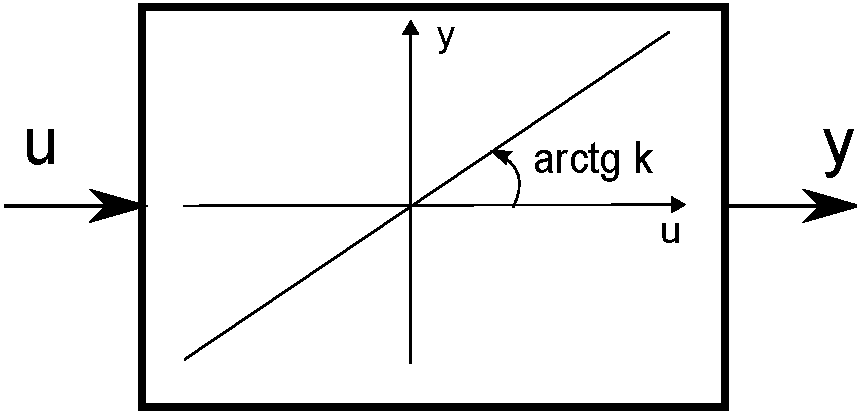
\includegraphics[width=8cm]{block_gain.pdf}
        \caption{Статическая характеристика П-звена}
        \centering
    \end{figure}
    % subsection звено_сау (end)
\subsection{Линеаризация} % (fold)
    Назначение САУ - это поддержание определенного заданного режима. Поэтому параметры, описывающие САУ, не должны сильно отличаться от заданного режима. Эта простая идея обычно позволяет проводить операцию линеаризации.
    \defi{\it Линеаризация} - построение приближенной линейной модели на основе более реалистичной нелинейной модели.
    Рассмотрим пример для уравнения 
    \eref{EQ_DYNAMIC}.
    Пусть заданный режим имеет вид
    \begin{equation}
        y = y^0, \dot y = \ddot y = 0, u=u^0, \dot u = 0, v=v^0.
    \end{equation}
    Тогда реальные параметры САУ можно записать в отклонениях как
    \begin{equation}
        y = y^0+\Delta y,\;\dot y = \dot{\Delta y},\;\ddot y = \ddot{\Delta y},\; u = u^0 + \Delta u,\; \dot u = \dot{\Delta u},\;v = v^0 + \Delta v,
    \end{equation}
    где переменные со знаком $\Delta$ достаточно малы.
    Тогда для функции 
    $F(y,\dot y, \ddot y, u, \dot u, v)$ 
    воспользуемся разложением в ряд Тейлора в точке 
    $(y^0, 0,0, u^0, 0, v^0)$:
    \begin{multline}
        F(y,\dot y, \ddot y, u, \dot u, v) = F^0 + \frac{\partial F}{\partial y} \Delta y +\frac{\partial F}{\partial \dot y} \dot{\Delta y}+ \frac{\partial F}{\partial \ddot y} \ddot{\Delta y} +\\  + \frac{\partial F}{\partial u} \Delta u + \frac{\partial F}{\partial \dot u } \dot{\Delta u} + \frac{\partial F}{\partial v} \Delta v + \ldots,
    \end{multline}
    где $F^0= 0$, многоточием обозначены члены с более высоким порядком малости.
    Отсюда получают линеаризацию уравнения 
    \eref{EQ_DYNAMIC} 
    вида
    \begin{equation}\label{EQ_LINEAR}
        a_2\ddot{\Delta y} + a_1 \dot{\Delta y} + a_0 \Delta y - b_1\dot{\Delta u} - b_0\Delta u - c_0 \Delta v = 0,
    \end{equation}
    где 
    $a_0 = \frac{\partial F}{\partial y}$, 
    $a_1 = \frac{\partial F}{\partial \dot y}$, $a_2 = \frac{\partial F}{\partial \ddot y}$, 
    $b_0 = -\frac{\partial F}{\partial u}$, 
    $b_1 = -\frac{\partial F}{\partial \dot u }$ и 
    $c_0 = -\frac{\partial F}{\partial v}$.
    Введем оператор дифференцирования: 
    $s = \frac{d}{dt}$.
    Тогда уравнение 
    \eref{EQ_LINEAR}
     примет вид (знаки $\Delta$ опущены)
    \begin{equation}
        a_2 s^2 y + a_1 s y + a_0 y = b_1 s u + b_0 u + c_0 v,
    \end{equation}
    что эквивалентно
    \begin{equation}
        Q(s) y = R_1(s)u + R_2(s)v,
    \end{equation}
    где 
    $Q(s) = a_2s^2 + a_1 s + a_0$ 
    называют {\it собственным оператором}, а 
    $R_1(s) = b_1s+b_0$ и 
    $R_2(s) = c_0$
     --- {\it операторами воздействия}.
    \defi{\it Собственный оператор} - дифференциальный оператор $Q(s)$ при выходной величине.
    \defi{\it Оператор воздействия} - дифференциальный оператор $R(s)$ при входной величине.
    % subsection линеаризация (end)
    % section уравнения_динамики_и_статистики (end)
\section{Преобразование Лапласа} % (fold)
    Для исследования и описания ОДУ часто используют преобразование Лапласа, так как оно сводит решение дифференциальных уравнений к алгебраическим операциям.
    \defi{\it Преобразованием Лапласа} называют отображение 
    $\LAP{\cdot}$ 
    функции 
    $x(t), t\in\BF{R}$
     в функцию 
    $X(s), s\in\BF{C}$
    , осуществляемое по правилу
    \begin{equation}
        X(s) = \LAP{x(t)} \stackrel{def}{=} \int\limits_0^\infty e^{-st} x(t) dt,
    \end{equation}
    где $x(t)$ --- исходная функция, $X(s)$ --- изображение по Лапласу, $s$~---~переменная преобразования Лапласа.
    Условия, при которых преобразование существует для $x(t)$:
    \begin{enumerate}
        \item $x(t)$ --- интегрируемая на любом конечном интервале функция;
        \item $x(t)\equiv0$ при $t < 0$;
        \item $\exists c, M > 0: |x(t)| < M e^{ct}, \forall t \ge 0$.
    \end{enumerate}
    Если $x(t)$ удовлетворяет всем вышеперечисленным свойствам, то её называют функцией-оригиналом.
\subsection{Обратное преобразование Лапласа} % (fold)
    Соотношение, определяющее по известному изображению его оригинал, называют {\it обратным преобразованием Лапласа}. 
    \begin{equation}
        x(t) = \INVLAP{X(s)} = \frac{1}{2\pi j} \int\limits_{\sigma-j\infty}^{\sigma + j\infty} X(s)e^{st} ds,
    \end{equation}
    где интегрирование ведется вдоль любой прямой 
    $\RE{s} = \sigma > c$, 
    где $с$ --- константа из условий существования преобразования Лапласа для $x(t)$.
% subsection обратное_преобразование_лапласа (end)
\subsection{Свойства преобразования Лапласа и примеры} % (fold)
    Пусть 
    $X(s) = \LAP{x(t)}$ и 
    $Y(s) = \LAP{y(t)}$.
    \begin{enumerate}
        \item Линейность. $\LAP{\alpha x(t) + \beta y(t)} = \alpha X(s) + \beta Y(s);$
        \item Дифференцирование оригинала. \\
            Если производная 
            $\dot x(t)$ 
            является функцией-оригиналом, то 
            $\LAP{\dot x(t)} = sX(s) - x(0);$
        \item Интегрирование оригинала.
            \begin{equation}
                \LAP{\int\limits_0^tx(\tau)d\tau} = \frac{X(s)}{s};
            \end{equation}
        \item Теорема запаздывания. Для любого $\tau>0$:
            \begin{equation}
                \LAP{x(t-\tau)} = e^{-\tau s}X(s);
            \end{equation}
        \item  Теорема о свертке (или об умножении изображений).\\
            Если $x(t)$ и $y(t)$ - оригиналы изображений, а $X(t)$ и $Y(t)$ - их изображения, то
            \begin{equation}
                X(s)\cdot Y(s) = \LAP{\int\limits_0^tx(\tau)y(t-\tau)d\tau} = \LAP{\int\limits_0^ty(\tau)x(t-\tau)d\tau};
            \end{equation}
            Интеграл в правой части называют {\it сверткой функций} $x_1(t)$ и $x_2(t)$, его обозначают $x_1(t) * x_2(t)$:
            \begin{equation}
                x_1(t)*x_2(t) = \LAP{\int\limits_0^t x_1(\tau) x_2(t-\tau) d{\tau}} = \LAP{\int\limits_0^t x_2(\tau) x_1(t-\tau)d\tau}.
            \end{equation}
            Поэтому 
            \begin{equation}
                X_1(s) * X_2(s) = L\{x_1(t) * x_2(t)\}
            \end{equation}
        \item Теорема о предельных значениях.
            \begin{enumerate}[label*={\arabic*}]
                \item 
                    $x(0) = \LAP{\lim\limits_{s\rightarrow\infty}sX(s)}$;
                \item Если существует 
                    $x(\infty) = \lim\limits_{t\rightarrow\infty} x(t)$, тогда 
                    $x(\infty) = \lim\limits_{s\rightarrow0} sX(s)$.
            \end{enumerate}
        \item Теорема разложения. \\
            Если изображение по Лапласу есть дробно-рациональная функция, т.е. 
            $X(s) = \frac{B(s)}{A(s)}$, где 
            $A(s)$ и $B(s)$ --- полиномы от $s$ и 
            $\deg A(s) > \deg B(s)$. 
            Тогда
            \begin{equation}
                x(t) = \sum_{k=1}^q\frac{1}{(n_k-1)!}\lim\limits_{s\rightarrow s_k} \frac{d^{n_k-1}}{d s^{n_k-1}} (X(s)(s-s_k)^{n_k}e^{ts}),
            \end{equation}
            где $s_k$ --- корни уравнения 
            $A(s)=0$, $n_k$ --- кратность $k$-го корня, $q$ --- количество различных корней.
            Когда $q=n$ (все корни простые), тогда
            \begin{equation}\label{eq:razl}
                x(t) = \sum^{n}_{k=1}\frac{B(s_k)}{A'(s_k)} e^{s_kt}.
            \end{equation}
    \end{enumerate}
    \examp Определить функцию $x(t)$, изображение которой имеет вид 
    $
        X(s) = \frac{1}{s (s+1)}.
    $\\
    {\bf Решение}\par
    В данном случае
    \begin{equation}
        B(s) = 1,\ A(s) = s (s+1),\ A'(s) = 2 s + 1.
    \end{equation}
    Полюсами функции $X(s)$ являются $s_1 = 0$, $s_2 = -1$, и они являются простыми. Поэтому, согласно формуле \eref{eq:razl} $x(t)=1-e^{-t}$
    \begin{table}
        \begin{center}
            \begin{tabular}{|c|c|c|}
            \hline 
            № & Оригинал $x(t)$ & Изображение $X(s)$\\ \hline
            1 & $\delta(t)$ & $1$ \\ \hline
            2 & $1(t)$ & $\frac{1}{s}$ \\ \hline
            3 & $1(t-\tau)$ & $\frac{1}{s} e^{-\tau s}$ \\ \hline
            4 & $t$ & $\frac{1}{s^2}$ \\ \hline
            5 & $t^n$ & $\frac{n!}{s^{n+1}}$ \\ \hline
            6 & $e^{-\alpha t}$ & $\frac{1}{s+\alpha}$ \\ \hline
            7 & $t e^{-\alpha t}$ & $\frac{1}{(s+\alpha)^2}$ \\ \hline
            8 & $t^n e^{-\alpha t}$ & $\frac{n!}{(s+\alpha)^{n+1}}$ \\ \hline
            9 & $\sin{\omega t}$ & $\frac{\omega}{s^2 + \omega^2}$ \\ \hline
            10 & $\cos{\omega t}$ & $\frac{s}{s^2+\omega^2}$ \\ \hline
            11 & $e^{-\alpha t} \sin{\omega t}$ & $\frac{\omega}{(s+\alpha)^2+\omega^2}$ \\ \hline
            12 & $e^{-\alpha t} \cos{\omega t}$ & $\frac{s+\alpha}{(s+\alpha)^2+\omega^2}$ \\ \hline
            \end{tabular}
            \caption{Изображения Лапласа для часто используемых функций}
        \end{center}
    \end{table}
    % subsection свойства_преобразования_лапласа_и_примеры (end)
\subsection{Передаточная функция в изображениях Лапласа} % (fold)
    Рассмотрим линейное уравнение с постоянными коэффициентами вида
    \begin{equation}\label{EQ_ODU}
    y^{(n)} + a_{n-1}y^{(n-1)} + \ldots + a_1 \dot y + a_0y = b_m u^{(m)} + \ldots + b_1 \dot u + b_0 u,
    \end{equation}
    при нулевых начальных условиях, т.е. 
    $y^{(n-1)} (0) = \ldots = \dot y(0) = y(0) = 0, u^{(m-1)} (0) = \ldots = \dot u(0) = u(0) = 0$
    Применяя к обеим частям равенства преобразование Лапласа, получим
    \begin{equation}\label{EQ_W}
    \left(s^n + \sum_{i=0}^{n-1}a_is^i\right) Y(s) = \left(\sum_{i=0}^{m}b_is^i\right) U(s),
    \end{equation}
    где $Y(s) = \LAP{y(t)}$, $U(s) = \LAP{u(t)}$. Разделив уравнение \eref{EQ_W} на полином в левой части, получим
    \begin{equation}  
        Y(s) = W(s)U(s),
    \end{equation}
    где 
    $W(s) = \frac{\beta(s)}{\alpha(s)}$, 
    $\alpha(s) = s^n + \sum_{i=0}^{n-1}a_is^i$ и 
    $\beta(s) = \sum_{i=0}^{m}b_is^i$.
    \defi{\it Передаточной функцией системы \eref{EQ_ODU} в изображениях Лапласа} называется отношение преобразований Лапласа входа и выхода системы при нулевых начальных условиях, причем отношение имеет наименьший порядок.
    Для системы, описываемой уравнением \eref{EQ_ODU}, передаточной функцией является дробно-рациональная функция $W(s)$, в которой были проведены сокращения общих множителей.
    \examp Дана система
    $$
        \ddot y - 2\dot y + y = \dot u - u.
    $$
    Найти передаточную функцию $W(s)$.
% subsection передаточная_функция_в_изображениях_лапласа (end)
\subsection{Передаточная функция в операторной форме} % (fold)
    Из записи уравнения \eref{EQ_ODU} в операторной форме вида
    \begin{equation}\label{EQ_ODU_SYM_1}
        A(s)y = B(s)u,
    \end{equation}
    где 
    $A(s) = s^n + \sum_{i=0}^{n-1}a_is^i$ и 
    $B(s) = \sum_{i=0}^{m}b_is^i$ --- ``составные'' операторы дифференцирования.
    Формально разделив \eref{EQ_ODU_SYM_1} на $A(s)$, получим
    \begin{equation}
        y(t) = W(s)u(t),
    \end{equation}
    где 
    $W(s) = \frac{B(s)}{A(s)}$ --- передаточная функция (ПФ) системы \eref{EQ_ODU} в операторной форме.
    Заметим, что ПФ в операторной форме и в изображениях Лапласа совпадают, если полиномы $A(s)$ и $B(s)$ не имеют общих корней. Однако ПФ в изображениях Лапласа всегда можно получить из ПФ в операторной форме, проведя сокращения числителя и знаменателя. Получить из ПФ в изображениях Лапласа ПФ в операторной форме не всегда возможно.
    \examp Определить передаточные функции звеньев, описываемых уравнениями:
    \begin{tasks}(2)
        \task $\dot y + y = u$
        \task $\ddot y - y = \dot u - u$
    \end{tasks}
    {\bf Решение.}
    В символической форме эти уравнения записываются в виде:
    \begin{tasks}(2)
        \task $(p+1) y = u$
        \task $(p^2-1) y = (p-1) u$
    \end{tasks}
    Их передаточные функции в операторной форме соответственно равны
    $$
        W_1(p)=\frac{1}{s+1}, \ W_2(p)= \frac{p-1}{p^2-1}
    $$
    Передаточные функции в изображениях Лапласа имеют вид
    $$
        \left.W_1(s)=W_1(p)\right\vert_{p=s} = \frac{1}{s+1}, \ 
        \left.W_2(s)=W_2(p)\right\vert_{p=s} = \frac{s-1}{s^2-1} = \frac{1}{s+1}.
    $$
% subsection передаточная_функция_в_операторной_форме (end)
\subsection{Временные функции: переходная и весовая функции} % (fold)
    Кроме дифференциальных уравнений и передаточных функций при описании и исследовании линейных систем используют переходные и импульсные переходные функции и их графики - временные характеристики.
    Для линейных систем справедлив {\it принцип суперпозиции \cite[стр. 35]{kim:uch}}. 

    \defi{\it Переходная функция} $h(t)$  - функция, описывающая реакцию системы (звена) на единичное ступенчатое воздействие при нулевых начальных условиях. 
    График переходной функции - кривую зависимости $h(t)$ от времени $t$ - называют {\it переходной} или {\it разгонной характеристикой}.
    \defi{\it Импульсная переходная (весовая)} функция $w(t)$ - функция, описывающая реакцию системы (звена) на единичное импульсное воздействие ($\sigma(t)$) при нулевых начальных условиях.\\ 
    График импульсной переходной функции - кривую зависимости функций w(t) от времени t - называют {\it импульсной переходной характеристикой}.
    Данные функции связаны соотношением - $w(t) = \frac{dh(t)}{dt}$.

% subsection временные_функции (end)
\subsection{ВФ и ПФ в изображениях Лапласа } % (fold)
    По определению ПФ имеем
    $$
        Y(s) = W(s)U(s).
    $$
    По определению переходной функции вход имеет вид 
    $u(t) = \IT{X}(t)$ 
    (а~$h(t) = y(t)$), а значит 
    $U(s) = \LAP{u(t)} = \frac{1}{s}$, поэтому
    $$
        Y(s) = \frac{W(s)}{s},
    $$
    откуда с помощью обратного преобразования Лапласа получаем 
    $h(t) = \INVLAP{\frac{W(s)}{s}}$.
    Аналогично для весовой функции: 
    $u(t) = \delta(t)$ 
    (a $\omega(t) = y(t)$), тогда $U(s)=1$. Получим, что
    $$
        Y(s) = W(s),
    $$
    откуда 
    $\omega(t) = \INVLAP{W(s)}$.
    Таким образом, имея хотя бы одну из функций ($h(t), \omega(t)$ или $W(s)$), можно восстановить оставшиеся.
% subsection ВФ и ПФ в изображениях Лапласа  (end)
% section преобразование_лапласа (end)
\section{Частотные функции} % (fold)
    Еще один распространенный способ описания динамических систем --- это {\it частотные функции}.
    Пусть дана ПФ $W(s)$. Функция 
    $W(j\omega), \omega\in\BF{R}$ 
    называется {\it частотной передаточной функцией} (ЧПФ), а переменная $\omega$ называется {\it частотой}.
    \defi{\it Частотная передаточная функция (ЧПФ)} - функция W(j), являющаяся комплекснозначной функцией от действительной переменной - частота. 
    Представим ЧПФ в виде
    $$
        W(j\omega) = U(\omega) + jV(\omega) = A(\omega)e^{j\phi(\omega)},
    $$
    где 
    $U(\omega)$ и $V(\omega)$ 
    --- {\it вещественная и мнимая частотные функции}, 
    $A(\omega) = |W(j\omega)| = \sqrt{U^2(\omega)+V^2(\omega)}$ 
    --- {\it амплитудная частотная функция}, 
    $\phi(\omega) = \arg{W(j\omega)}$ (при 
    $|\arg{W(j\omega)}| \le \frac{\pi}{2}$ верно 
    $\phi(\omega) = arctg\left(\frac{V(\omega)}{U(\omega)}\right)$) 
    --- фазовая частотная функция.
    График для каждой частотной функции называется {\it характеристикой}.\par
    Если линейная стационарная система устойчива, то входные гармонические сигналы после окончания переходного процесса переходят в гармонические сигналы с той же частотой, но со сдвигом по фазе и другой амплитудой. Это преобразование характеризует частотная функция 
    $W(j\omega)$.
    Пусть вход 
    $u(t) = u_0 \cos(\omega t + \alpha)$ 
    --- гармонический сигнал. Найдем выход $y(t)$ линейной системы вида
    \begin{equation}\label{EQ_ODU_SYM_2}
        Q(s)y = R(s)u,
    \end{equation}
    при гармоническом воздействии (здесь 
    $Q(s) = s^n + \sum_{i=0}^{n-1}a_is^i,\quad R(s) = \sum_{i=0}^{m}b_is^i, \quad s=\frac{d}{dt}$). 
    Пользуясь {\it принципом суперпозиции} для последнего уравнения, найдем выход $y(t)$ как сумму двух выходов при воздействиях 
    $u_1(t) = u_0e^{j(\omega t+\alpha)}$ и 
    $u_2(t) = u_0e^{-j(\omega t+\alpha)}$ (заметим, 
    $u(t) = \frac{u_1(t)+u_2(t)}{2}$).\par
    Тогда в правой части уравнения имеем
    $$
        R(s)u_1(t) = u_1(t)R(j\omega),\quad R(s)u_2(t) = u_2(t)R(-j\omega).
    $$
    Решения будем искать в виде $y_1(t) = A u_0e^{j(\omega t + \alpha + \phi)} = Ae^{j\phi}u_1(t)$ и $y_2(t) = A u_0e^{-j(\omega t + \alpha + \phi)} = Ae^{-j\phi}u_2(t)$, где $\phi$ и $A$ --- параметры, подлежащие определению.

    В левых частях уравнений получим $Q(s)y_1(t) = Ae^{j\phi}u_1(t)Q(j\omega)$ и $Q(s)y_2(t) = Ae^{j\phi}u_2(t)Q(-j\omega)$. Таким образом, имеем два равенства
    $$
        Ae^{j\phi} u_1(t)Q(j\omega) = u_1(t)R(j\omega),\quad Ae^{-j\phi} u_2(t)Q(-j\omega) = u_2(t)R(-j\omega),
    $$
    что эквивалентно
    $$
        Ae^{j\phi} = W(j\omega),\quad Ae^{-j\phi} = W(-j\omega),
    $$
    откуда следует, что 
    $$
        A = |W(j\omega)| = |W(-j\omega)|
    $$ 
    и 
    $\phi = \arg W(j\omega) = -\arg W(-j\omega)$. В итоге,
    $$
        y_1(t) = Au_0e^{j(\omega t + \alpha + \phi)},\quad
        y_2(t) = Au_0e^{-j(\omega t + \alpha + \phi)}.
    $$
    Следовательно, $y(t) = \frac{y_1(t)+y_2(t)}{2} = u_0|W(j\omega)| \cos(\omega t + \alpha + \arg W(j\omega))$.

    Заметим, что найденное решение $y(t)$ является вынужденной составляющей решения уравнения \eref{EQ_ODU_SYM_2}.  В силу того, что в выкладках выше используются ПФ в преобразованиях Лапласа, начальные условия нулевые.

    Кроме вынужденной составляющей в решении есть свободные колебания, которые определяются из начальных условий и полинома $Q(s)$. Это означает, что в реальных системах такое преобразование гармонического сигнала будет явно видно только через некоторое время, т.е. после окончания {\it переходного процесса}. (Это можно увидеть при моделировании линейной системы с входным гармоническим сигналом.)
% section частотные_функции (end)
\section{Основные типы элементарных звеньев} % (fold)

\begin{description}
\item[Пропорциональное звено] % (fold)
    Пропорциональное звено: $W(s)=k$.  
    $W(j\omega) = k,\; A(\omega) = |k|,\; \phi(\omega) = 0,\; h(t) = k,\; \omega(t) = k\delta(t);$
% item[пропорциональное_звено (end)
\item[Дифференциальное звено] % (fold)
    Дифференциальное звено: $W(s) = ks$.
    $$
        W(j\omega) = kj\omega,\; A(\omega) = |k|\omega, \; \phi(\omega) = \frac{\pi}{2},\; h(t) = k\delta(t),\; \omega(t) = k\dot\delta(t);
    $$
% % item[дифференциальное_звено (end)
\item[Интегрирующее звено] % (fold)
    Интегрирующее звено: $W(s) = \frac{k}{s}$.
    $$
        W(j\omega) = -\frac{k j}{\omega},\; A(\omega) = \frac{|k|}{\omega},\; \phi(\omega) = -\frac{\pi}{2},\; h(t) = kt,\; \omega(t) = k;
    $$
% % item[интегрирующее_звено (end)
\item[Апериодическое звено] % (fold)
    Апериодическое звено: $W(s) = \frac{k}{Ts+1},\; T>0$.
    $$
        \begin{aligned}
            W(j\omega) = \frac{k}{jT\omega+1},\; &A(\omega) = \frac{|k|}{\sqrt{(T\omega)^2+1}},\; \phi(\omega) = -\arctg(\omega T),\\ h(t) = k(1-&e^{-\frac{t}{T}}),\; \omega(t) = \frac{k}{T}e^{-\frac{t}{T}};
        \end{aligned}
    $$
% % item[апериодическое_звено (end)
\item[Колебательное звено] % (fold)
    Колебательное звено: $W(s) = \frac{k}{T^2s^2+2\xi Ts+1},\; T>0,\; 0 < \xi < 1.$
    $$
        \begin{aligned}
            W(j\omega) &= \frac{k}{1-T^2\omega^2 +j2\xi T\omega},\\
            A(\omega) &= \frac{|k|}{\sqrt{(1-(T\omega)^2)^2 + (2\xi T\omega)^2}},\\
            \phi(\omega) &=
            \begin{cases}
                -\arctg(\frac{2\xi T\omega}{1-(T\omega)^2}) & 1 \ge (T\omega)^2,\\
                -\pi+\arctg(\frac{2\xi T\omega}{(T\omega)^2-1}) & 1 < (T\omega)^2,
            \end{cases}\\
            h(t) &= k\left[1-\frac{\sqrt{\alpha^2+\beta^2}}{\beta} e^{-\alpha t} \sin{(\beta t+\varphi_0)}\right],\\
            \omega(t) &= \frac{k (\alpha^2 + \beta^2)}{\beta} e^{-\alpha t} \sin{\beta  t},
        \end{aligned}
    $$
    $$
        \text{где } \alpha = \frac{\zeta}{T},\ \beta=\frac{\sqrt{1-\zeta^2}}{T},\ \varphi_0=arctg{\frac{\sqrt{1-\zeta^2}}{\zeta}}.
    $$
% item[колебательное_звено (end)
\item[Звено чистого запаздывания] % (fold)

    Передаточная функция звена: $W(s) = ke^{-\tau s},\; \tau > 0$. Функции описывающие её
    $$
        \begin{aligned}
            W(j\omega) &= ke^{-j\tau\omega},\\
            A(\omega) = k,&\; \phi(\omega) = -\tau\omega,\\
            h(t) = k\IT{X}(t-\tau),&\; \omega(t) = k\delta(t-\tau).
        \end{aligned}
    $$

    Это классический способ описания чистого или транспортного запаздывания в системе: воздействие сигнала происходит не в тот же момент, а через некоторое время $\tau$.
\end{description}

\section{Структурные схемы и дифференциальные уравнения систем управления}

    \defi{\it Структурной схемой} системы управления называют графическое изображение её математической модели (ММ) в виде прямоугольников и кругов, обозначающих звенья её математической модели, с указанием входов и выходов. Причем кругами обозначают только сумматоры --- звенья, которые имеют не менее двух входов и один выход и в которых происходит сложение или вычитание входных сигналов.

    \begin{figure}[h]
        \centering
        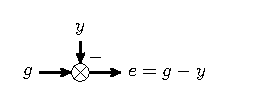
\includegraphics[width=6.5cm]{sum_minus.pdf}
        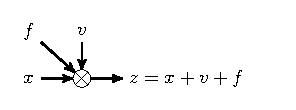
\includegraphics[width=6.5cm]{sum_three.pdf}
        \caption{Примеры структурных схем}
        \centering
    \end{figure}

\subsection{Преобразование структурных схем}

    Как любое другое звено, сумматор обладает ПФ. Для первого рисунка это передаточная функция с двумя входами и одним выходом вида
    $$
        W(s) =
        \begin{pmatrix}
            W_{ye}(s)\\
            W_{ge}(s)
        \end{pmatrix}^T =
        \begin{pmatrix}
            -1\\
            1
        \end{pmatrix}^T.
    $$
    Соответственно, получаем 
    $e = W(s)\begin{pmatrix}y\\g\end{pmatrix} = -y+g$.

    Для второго рисунка это
    $$
        W(s) =
        \begin{pmatrix}
            W_{vz}(s)\\
            W_{xz}(s)\\
            W_{fz}(s)
        \end{pmatrix}^T =
        \begin{pmatrix}
            1\\
            1\\
            1
        \end{pmatrix}^T.
    $$
    Соответственно, 
    $z = W(s) \cdot (v,\; x,\; f)^T= v+x+f$.

    \defi{\it Последовательное соединение} - соединение, при котором выходная переменная предшествующего звена является входной переменной последующего звена.
    \begin{figure}[h]
        \centering
        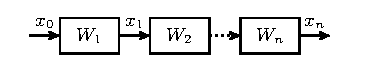
\includegraphics[width=6.5cm]{series_connection.pdf}
        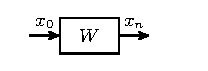
\includegraphics[width=3.5cm]{sconnection_whole.pdf}
        \caption{Примеры структурных схем}
        \centering
    \end{figure}
    При последовательном соединении ПФ между сигналами $x_0$ и $x_n$ вычисляется по формуле 
    $W = W_1\cdot W_2\cdot \ldots\cdot W_n$.
    \defi{\it Параллельное соединение} - соединение, при котором на входы всех звеньев подается одно и то же воздействие, а их выходные переменные складываются.
    \begin{figure}[h]
        \begin{minipage}[h]{0.39\linewidth}
            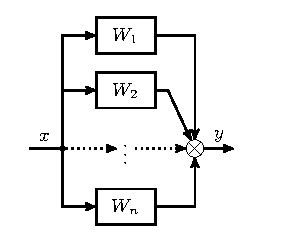
\includegraphics[width=5cm]{parallel_connection.pdf}
        \end{minipage}
        \begin{minipage}[h]{0.59\linewidth}
            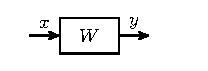
\includegraphics[width=5cm]{pconnection_whole.pdf}\\
            При параллельном соединении ПФ вычисляется по формуле 
            $W = W_1+W_2+\ldots \hm+ W_n$.
        \end{minipage}
    \end{figure}
    \defi{\it Обратное соединение} - соединение двух звеньев, при котором выход звена прямой цепи подается на вход звена обратной связи, выход которого складывается с входом первого звена.
    \begin{figure}[h]
        \begin{minipage}[h]{0.39\linewidth}
            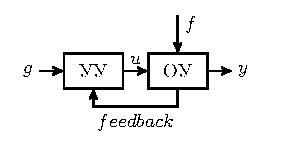
\includegraphics[width=5.5cm]{feedback.pdf}
        \end{minipage}
        \begin{minipage}[h]{0.60\linewidth}
            Если разомкнуть цепь у сумматора после блока $W_2$, получим цепь последовательно соединенных звеньев с передаточной функцией 
            $W_{\text{р}}\hm = W_1 \cdot W_2$, 
            называемой {\it передаточной функцией размокнутого контура}.
        \end{minipage}
    \end{figure}

    Легко найти звено, которое описывает такое обратное соединение, из следующих уравнений (записано для {\it отрицательной обратной связи}):
    $$
        y = W_1 e, \quad e = g- W_2 y.
    $$
    Откуда $y = W_{yg}g$, где
    $$
        W_{yg} = \frac{W_1}{1+W_1 W_2}.
    $$
    Для положительной обратной связи $W_{yg}$ определяется аналогично.\\\\
    {\bf Перенос сумматора}. Перенос сумматора бывает двух видов: по ходу сигнала и против хода сигнала. В первом случае добавляется звено с передаточной функцией, равной передаточной функции звена, через которое переносится сумматор.

    \begin{figure}[h]
        \begin{minipage}[h]{0.45\linewidth}
            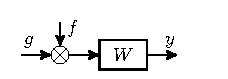
\includegraphics[width=5.5cm]{trans_sum_direct_before.pdf}
        \end{minipage}
        $\Longrightarrow$
        \begin{minipage}[h]{0.45\linewidth}
            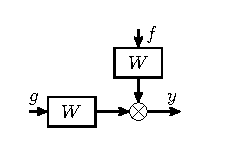
\includegraphics[width=5.5cm]{trans_sum_direct_after.pdf}
        \end{minipage}
        \caption{Выходной сигнал $y$ при таких преобразованиях остается неизменным.}
    \end{figure}
    При переносе сумматора против хода сигнала добавляется звено с передаточной функцией, равной обратной передаточной функции звена, через которое переносится сумматор.  
    \begin{figure}[h]
        \begin{minipage}[h]{0.45\linewidth}
           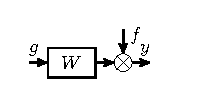
\includegraphics[width=5.5cm]{trans_sum_indirect_before.pdf}
        \end{minipage}
        $\Longrightarrow$
        \begin{minipage}[h]{0.45\linewidth}
            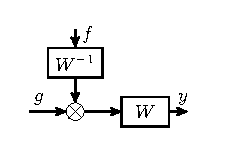
\includegraphics[width=5.5cm]{trans_sum_indirect_after.pdf}
        \end{minipage}
    \end{figure}\\
    {\bf Перенос узла}. Перенос узла, как и сумматора, бывает двух видов: по ходу сигнала и против хода сигнала. При переносе узла по ходу сигнала добавляется звено с передаточной функцией звена, равной обратной передаточной функции звена, через которое переносится узел.
    \begin{figure}[h]
        \begin{minipage}[h]{0.45\linewidth}
            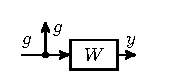
\includegraphics[width=5.5cm]{trans_branch_direct_before.pdf}
        \end{minipage}
    $\Longrightarrow$
        \begin{minipage}[h]{0.45\linewidth}
            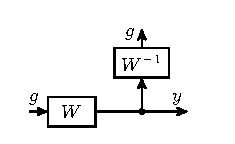
\includegraphics[width=5.5cm]{trans_branch_direct_after.pdf}
        \end{minipage}
        \caption{Аналогично, выходной сигнал $y$ при таких преобразованиях остается неизменным.}
    \end{figure}

    При переносе узла против хода  добавляется звено с передаточной функцией звена, равной передаточной функции звена, через которое переносится узел. 
    \begin{figure}[h]
        \begin{minipage}[h]{0.45\linewidth}
            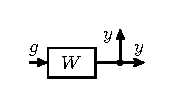
\includegraphics[width=5.5cm]{trans_branch_indirect_before.pdf}
        \end{minipage}
        $\Longrightarrow$
        \begin{minipage}[h]{0.45\linewidth}
            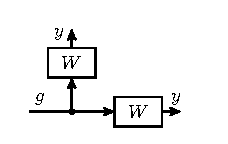
\includegraphics[width=5.5cm]{trans_branch_indirect_after.pdf}
        \end{minipage}
    \end{figure}\\
    {\bf Перестановка сумматоров и узлов}. Перестановка двух сумматоров соответствует перестановке одного сумматора через другой  и подчиняется правилу переноса сумматора через звено.
    \begin{figure}[h]
        \begin{minipage}[h]{0.45\linewidth}
            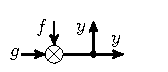
\includegraphics[width=5.5cm]{trans_sum_branch_before.pdf}
        \end{minipage}
        $\Longrightarrow$
        \begin{minipage}[h]{0.45\linewidth}
            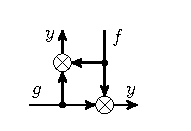
\includegraphics[width=5.5cm]{trans_sum_branch_after.pdf}
        \end{minipage}
    \end{figure}
    \begin{figure}[h]
        \begin{minipage}[h]{0.45\linewidth}
            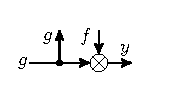
\includegraphics[width=5.5cm]{trans_branch_sum_before.pdf}
        \end{minipage}
    $\Longrightarrow$
        \begin{minipage}[h]{0.45\linewidth}
            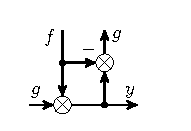
\includegraphics[width=5.5cm]{trans_branch_sum_after.pdf}
        \end{minipage}
    \end{figure}\\

\subsection{Вычисление передаточной функции одноконтурной и многоконтурной систем}

    \defi Замкнутая система называется {\it одноконтурной}, если при ее размыкании в какой-либо точке замкнутого контура получается цепь (схема) без параллельных и обратных соединений.

    \begin{figure}[h]
        \begin{minipage}[h]{0.29\linewidth}
            Рассмотрим пример.
            \vspace{3cm}
        \end{minipage}
        \begin{minipage}[h]{0.70\linewidth}
            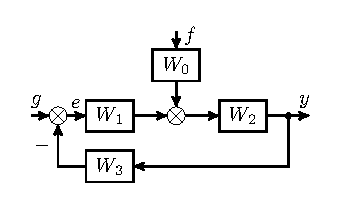
\includegraphics[width=9.5cm]{one_contour_exmpl.pdf}
        \end{minipage}
    \end{figure}

    {\bf Правило вычисления передаточной функции замкнутой одноконтурной системы}. 
    Передаточная функция одноконтурной системы относительно внешнего воздействия (входа) $u$ и выхода $х$ равна передаточной функции прямой цепи, деленной на единицу минус передаточная функция контура: $W_{xu}=\frac{W_\text{п}}{1-W_\text{к}}$.

    Тогда передаточная функция системы относительно входа $g$ и выхода $y$ 
    $$W_{gy}=\frac{W_1*W_2}{1+W_1*W_2*W_3},$$
    а для входа $f$ и выхода $e$ 
    $$W_{fe}=\frac{-W_0*W_2*W_3}{1+W_1*W_2*W_3}.$$

    \defi Замкнутая система называется {\it многоконтурной}, если при ее размыкании в какой-либо точке замкнутого контура получается цепь,содержащая параллельное, или обратное, или оба соединения. Многоконтурная система бывает двух видов: с перекрестными связями и без перекрестных связей.
    Многоконтурная система {\it не имеет перекрестных связей}, если любые два контура, образованные параллельными или обратными соединениями, не имеют общих участков или если какие-либо два контура имеют общий участок, то один из них вложен внутрь другого.
    \begin{figure}[h]
        \begin{minipage}[h]{0.19\linewidth}
            Рассмотрим пример.
            \vspace{3cm}
        \end{minipage}
        \begin{minipage}[h]{0.80\linewidth}
            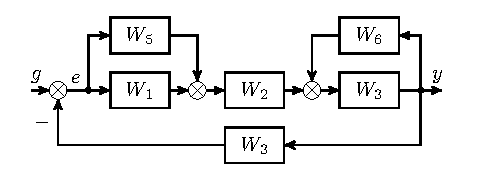
\includegraphics[width=9.5cm]{many_contour_no_cross_exmpl.pdf}
        \end{minipage}
    \end{figure}\\
    Многоконтурная система имеет {\it перекрестные связи}, если она содержит два контура, которые имеют общий участок, и при этом ни один из них не вложен внутрь другого.
    \begin{figure}[h]
        \begin{minipage}[h]{0.19\linewidth}
            Рассмотрим пример.
            \vspace{3cm}
        \end{minipage}
        \begin{minipage}[h]{0.80\linewidth}
            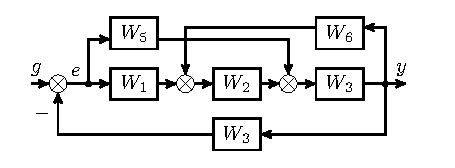
\includegraphics[width=9.5cm]{many_contour_cross_exmpl.pdf}
        \end{minipage}
    \end{figure}

\section{Основные способы математического описания САУ}
    \begin{enumerate}
        \item ОДУ:
            $$
                y^{(n)}+\sum_{i=0}^{n-1}a_iy^{(i)}=\sum_{i=0}^{m}b_iu^{(i)},\; m \le n;
            $$
        \item ПФ (в изображениях Лапласа и в операторной форме):
            $$
                W(s) = \frac{\sum_{i=0}^{m}b_is^i}{s^n+\sum_{i=0}^{n-1}a_is^{i}} = \frac{\beta(s)}{\alpha(s)};
            $$
        \item Временные функции: $h(t)$ и $\omega(t)$;
        \item Система в пространстве состояний (ПС): ?
    \end{enumerate}

    \begin{figure}[!hb]
        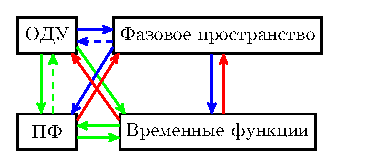
\includegraphics[width=9cm]{all_desc.pdf}
        \caption
        {    
            {\\\color{blue} Синий цвет}: переходы, которые будут рассмотрены.\\
            {\color{red} Красный цвет}: переходы, которые не будут рассматриваться в курсе.\\
            {\color{green} Зеленый цвет}: переходы, которые уже были рассмотрены.\\
            Прерванная линия означает, что переход возможен при определенных условиях.
        }
    \end{figure}
    \FloatBarrier
% \clearpage

\subsection{Описание системы в фазовом пространстве}
    
    Линейный ОУ может быть описан системой дифференциальных уравнений вида
    \begin{equation}\label{ST_DS}
        \begin{cases}
            \dot x = Ax+bu& x\in\BF{R}^{n},u\in\BF{R},\\
            y = cx +d u& y\in\BF{R},
        \end{cases}
    \end{equation}
    где $u(t)$ и $y(t)$ --- назначаемое управление и выход, $x(t)$ --- вектор состояния системы или фазовый вектор, матрицы $A,b$ и $c$ соответствующих размерностей, $d$ --- число (в основном везде будем полагать, что $d=0$). Такое описание называют описанием системы в фазовом пространстве.

    Если ОУ линейный нестационарный, то матрицы в \eref{ST_DS} зависят от времени: $A=A(t), b=b(t)$ и $c=c(t)$.

    На второй лекции был рассмотрен перевернутый маятник и его описание в пространстве состояний.

\subsection{Переход от ОДУ к ПС}

    Пусть дано описание ОУ в виде ОДУ  
    $y^{(n)}+\sum_{i=0}^{n-1}a_iy^{(i)}=\sum_{i=0}^{m}b_iu^{(i)},\; m \le n$. 
    Определим алгоритм перехода от ОДУ к описанию в ПС~\eref{ST_DS}.

    Рассмотрим этот переход для случая $n=m=2$. Тогда имеем ОДУ
    \begin{equation}\label{ODU_2}
        \left\{
        \begin{aligned}
            &\ddot y + a_1 \dot y + a_0 y = b_2 \ddot{u} + b_1 \dot u + b_0 u,\\
            &\dot y(0) = y_1,\quad y(0) = y_0,
        \end{aligned}\right.
    \end{equation}
        и требуется перейти к ПС
    \begin{equation}\label{STDS_2}
        \left\{
        \begin{aligned}
            \dot x &= Ax + ku,\\
            y &= cx + du,\\
            x_1(0) &= x_{10},\quad x_2(0) = x_{20},
        \end{aligned}
        \right.
    \end{equation}
    где 
    $A\in\BF{R}^{2\times2}, k, c^T\in\BF{R}^{2\times1}$ 
    и 
    $d,x_{10}, x_{20}\in\BF{R}$ --- 
    параметры, подлежащие определению.

    Выбор параметров $A,b,c$ и $d$ может быть разнообразным, но при этом выходы в описаниях \eref{ODU_2} и \eref{STDS_2} должны совпадать. Рассмотрим один из способов.

    Оказывается, что матрицу $A$ можно выбрать в виде матрицы Фробениуса характеристического полинома ОДУ \eref{ODU_2} (
    $\alpha(s) = s^2+a_1s+a_0$) , 
    т.е.
    $$
        A =
        \begin{pmatrix}
            0&    1\\
            -a_0& -a_1
        \end{pmatrix},
    $$
    а $с = (1\; 0)$. Тогда описание \eref{STDS_2} принимает вид
    \begin{equation}\label{EQ1}
        \left\{
        \begin{aligned}
            \dot x_1 &= x_2 + k_1 u,\\
            \dot x_2 &= -a_0x_1-a_1x_2+k_2u\\
            y &= x_1 + du,\\
            x_1(0) &= x_{10},\quad x_2(0) = x_{20}.
        \end{aligned}
        \right.
    \end{equation}

    Чтобы определить параметры $k_1,k_2$ и $d$, выведем уравнение, связывающее $y$ и $u$. Для этого в \eref{EQ1} выразим $x_1$ и $x_2$ через $y$ и $u$:
    $x_1 = y - du$, 
    отсюда 
    $x_2 = \dot y - d\dot u -k_1 u$. 
    В результате получаем уравнение для $y$ и $u$:
    $$
        \ddot y - d \ddot u -k_1\dot u = -a_0 (y-du)-a_1(\dot y - d \dot u - k_1 u)+k_2u.
    $$
    Сгруппируем и приведем подобные:
    $$
        \ddot y +a_1\dot y + a_0 y = d\ddot u + (k_1+a_1d)\dot u + (a_0 d + a_1k_1+k_2)u.
    $$
    Это уравнение должно совпадать с исходным уравнением \eref{ODU_2}, т.е.
    $d = b_2,\; k_1 + a_1d = b_1,\; a_0 d+a_1k_1+k_2 = b_0$. 
    Отсюда окончательные выражения:
    $$
        \left\{
        \begin{aligned}
            d&=b_2,\\
            k_1 &= b_1 - a_1b_2,\\
            k_2 &= b_0 - a_0 b_2 - a_1 (b_1-a_1b_2).
        \end{aligned}
        \right.
    $$

    Таким образом, динамика у уравнения \eref{ODU_2} и у системы уравнений \eref{STDS_2} одинакова, однако если не совпадают начальные условия, то выходы все еще будут различны. Поэтому необходимы {\it условия согласования} начальных условий.

    Повторно пользуясь выражениями 
    $x_1 = y - du$ 
    и 
    $x_2 = \dot y - d\dot u -k_1 u$, 
    получим условия согласования
    $$
        \begin{aligned}
            x_{10} &= y_0- b_2 u(0),\\
            x_{20} &= y_1-b_2\dot u (0) - (b_1-a_1b_2)u(0).
        \end{aligned}
    $$

\subsection{Переход от ПС к ПФ. Инвариантность формы 
ПФ при невырожденном преобразовании вектора состояния}

    Как вычислить ПФ, если система дана в виде указанном ниже?
    $$
        \left\{
        \begin{aligned}
            \dot x &= Ax+bu,\\
            y&= cx.
        \end{aligned}
        \right.
    $$
    Как и в случае с ОДУ $n$-го порядка, чтобы получить ПФ в изображениях по Лапласу, достаточно взять преобразование от всех уравнений при нулевых начальных условиях. Тогда в обозначениях 
    $X(s)=\LAP{x(t)}, Y(s)=\LAP{y(t)}, U(s) = \LAP{u(t)}$ 
    получим
    $$
        \left\{
        \begin{aligned}
            Xs &= AX+bU,\\
            Y &= cX,
        \end{aligned}
        \right.
    $$
    откуда получаем 
    $X(s) = (sI-A)^{-1}b U(s)$ 
    и 
    $Y(s) = c(sI-A)^{-1}b U(s)$. 
    Последнее соотношение по определению ПФ означает, что
    $$
        W(s) = c (sI-A)^{-1}b = \frac{\beta(s)}{\alpha(s)}.
    $$

    Запись в пространстве состояний содержит ``внутреннюю'' переменную $x(t)$, фазовый вектор. Это даёт возможность выбирать эту переменную в некоторых пределах, например, от $x$ можно перейти к $z=Mx$, где 
    $\det M \neq 0,\quad M\in\BF{R}^{n\times n}$. 
    При этом выход $y$ и вход $u$ системы не изменятся, но изменятся матрицы $A, b$ и $c$. Домножив первое уравнение на $M$ и сделав замену 
    $x=M^{-1}z$, 
    получим:
    $$
        \left\{
        \begin{aligned}
            \dot z &=M AM^{-1}z+Mbu,\\
            y&= cM^{-1}z.
        \end{aligned}
        \right.
    $$
    В новом фазовом пространстве имеем
    $$
        \left\{
        \begin{aligned}
            \dot z &= \overline{A}z+\overline{b}u,\\
            y&= \overline{c}z,
        \end{aligned}
        \right.
    $$
    где 
    $\overline{A} = M AM^{-1},\; \overline{b} = Mb$ 
    и 
    $\overline{c}= cM^{-1}$.

    Вычислим ПФ в новом фазовом пространстве:
    \begin{multline*}
        W(s) = \overline{c}(sI-\overline{A})^{-1}\overline{b} = cM^{-1}(sI-MAM^{-1})^{-1}Mb = \\
        = c M^{-1} (sMM^{-1} - MAM^{-1})^{-1}Mb = c M^{-1}(M(sI-A)M^{-1})^{-1}Mb = \\
        =c(sI-A)^{-1}b.
    \end{multline*}

    Это означает инвариантность ПФ относительно невырожденных преобразований в фазовом пространстве.

\subsection{Формулы вычисления реакции системы}

    В ПС существует удобная формула для выражения реакции системы, которая опирается на формулу Коши для решения линейной системы уравнений. Для уравнения 
    $\dot x = Ax + bu, x(0) = x_0$ 
    она принимает вид
    $$
        x(t) = e^{At}x_0 + \int\limits_{0}^{t} e^{A(t-\tau)}bu(\tau)d\tau,
    $$
    где 
    $e^{At} = I+\frac{1}{1!}At + \frac{1}{2!}(At)^{2} + \ldots$ --- 
    матричная экспонента.
    Тогда реакция системы выражается как
    $$
        y(t) = ce^{At}x_0 + c\int\limits_{0}^{t} e^{A(t-\tau)}bu(\tau)d\tau.
    $$

    Для ПФ выполнено 
    $Y(s) = W(s)U(s)$. 
    После применения обратного преобразования Лапласа при нулевых начальных условиях, $x_0=0$, к последнему соотношению получим
    $$
        y(t) = \IT{L}^{-1}\{W(s)U(s)\} = \int\limits_{0}^t\omega(t-\tau)u(\tau)d\tau.
    $$

    Таким образом, свертка весовой функции и входного воздействия равна реакции системы.

\subsection{Переход от ПС к временным функциям}

    Для ПФ выполнено 
    $Y(s) = W(s)U(s)$. 
    После применения обратного преобразования Лапласа при нулевых начальных условиях, $x_0=0$, к последнему соотношению получим
    $$
        y(t) = \IT{L}^{-1}\{W(s)U(s)\} = \int\limits_{0}^t\omega(t-\tau)u(\tau)d\tau.
    $$

    Таким образом, свертка весовой функции и входного воздействия равна реакции системы.

%chapter математическое_описание_непрерывных_систем_уравнений (end)
\end{document}